\chapter{Конструкторский раздел}

В данном разделе будут описаны особенности написания программ для графических процессоров, 
будут разработаны алгоритмы, выбранные для решения поставленной задачи.

\section{Особенности написания программ для графических процессоров}

Написание программ для графических процессоров имеет следующие особенности:
\begin{itemize}
    \item получение входных данных в виде последовательности графических примитивов;
    \item разделение программы на несколько этапов;
    \item использование специального языка программирования;
    \item отсутствие прямого доступа к памяти;
    \item высокая вычислительная стоимость условных переходов.
\end{itemize}

Входными данными являются треугольники. При отрисовке сцены используется два треугольника,
определяющих прямоугольник видимости экрана.
Программы, называемые шейдерами (англ. Shader), конвеера (англ. Pipeline) 
графического процессора деляется на несколько этапов. Двумя основными этапами, 
без которых отрисовка не может быть выполнена, это этапы выполнения вершинного (англ. Vertex) и 
фрагментного (англ. Fragment) шейдеров. Вершинный шейдер выполняется для каждой из вершин один
раз, и его результаты линйеного интерполируются. Фрагментный шейдер
выполняется для каждого пикселя экрана и выполняет подсчет цвета этого пикселя.

\section{Разработка алгоритмов}

\subsection{Алгоритм трассировки лучей}

На рисунке~\ref{img:app_algo} приведена схема алгоритма работы программы.
$MAX\_BOUNCE\_COUNT$ -- это целочисленная константа, обозначающая максимальное число
отскоков одного луча. Под цветом понимается
трехмерный вектор в формате RGB в диапозоне $[0, 1)$. $rgb(0,0,0)$ -- функция черного цвета. 

\begin{figure}[H]
	\centering
	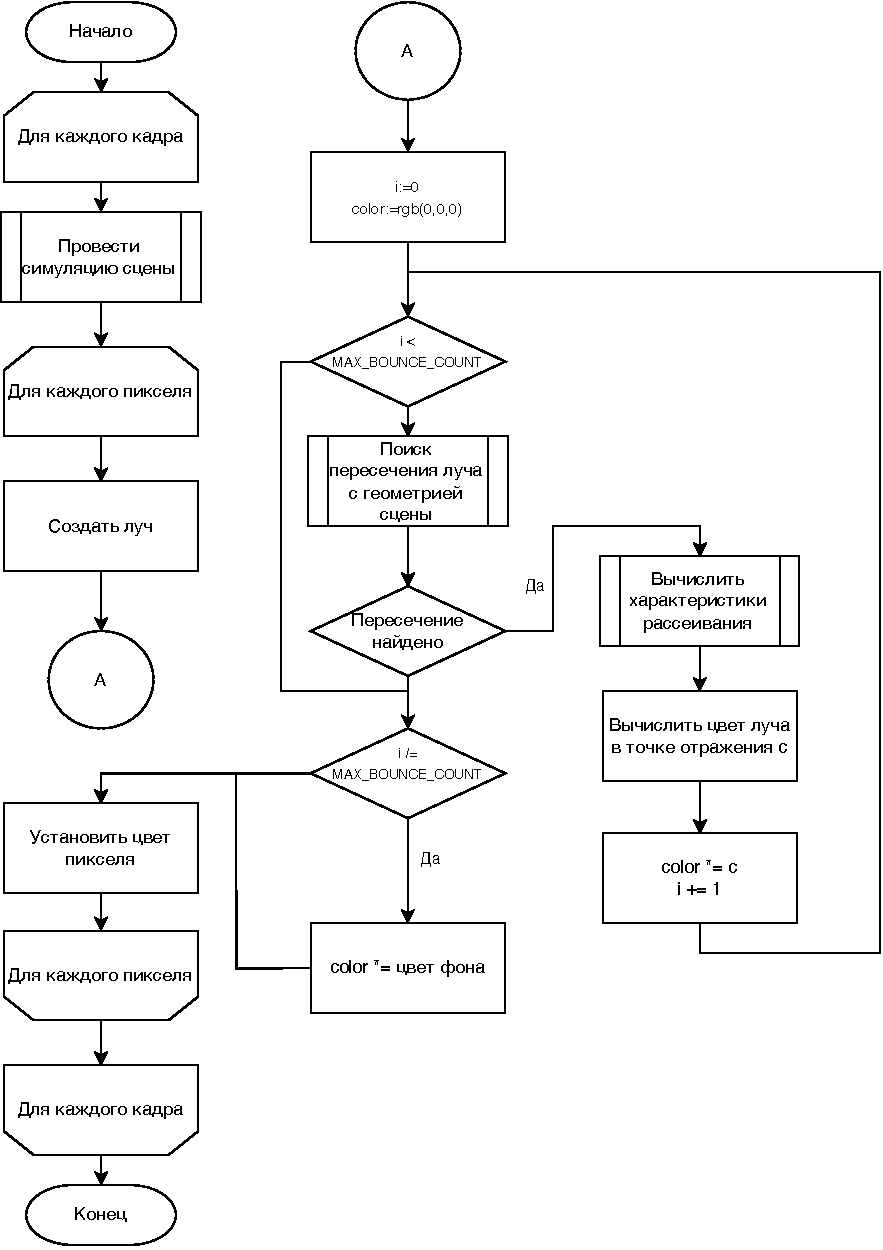
\includegraphics[width=120mm]{inc/pdf/app_algo}
	\caption{Схема алгоритма отрисовки}
	\label{img:app_algo}
\end{figure}

Алгоритм трассировки лучей реализуется в фрагментном шейдере.
Вычисление вектора направления луча производится в вершинном
шейдере и линейно интерполируется между всеми пикселями. В силу этого 
в фрагметных шейдерах необходимо произвести нормализацию вектора направления луча
перед его использованием.

Для передачи информации о камере используются две квадратных матрицы размерности 4: матрица проекции камеры и матрица вида камеры. Матрица вида камеры содержит информацию о том, 
как точка из пространства сцены преобразуется в пространство камеры. Матрица проекции 
содержит информацию о том, как точка из пространства камеры преобразуется в пространство 
изображения. Разделения преобразования на две части позволяет уменьшить число вычислений 
в случаях, когда вид меняется, а проекция остается неизменной.

В листинге~\ref{lst:trace} приведен псевдокод вершинного шейдера, выполняющий вычисление
координаты начала луча и вектора его направления.

\begin{lstlisting}[caption={Вычисление координаты начала луча и вектора его направления},label={lst:trace},frame=single]
vec4 t1 = inverse(projection_matrix) * vec4f(position, -1.0, 1.0);
vec4 t2 = view_matrix * vec4f(t1.xyz, 0.0);
vec3 ray_direction = t2.xyz;
vec3 ray_origin = vec3(view_matrix[3][0], view_matrix[3][1], view_matrix[3][2]);
\end{lstlisting}

\subsection{Алгоритм кеширования обратной репроекции}

Временная обратная репроекция -- это процесс отображения ранее сгенерированного кадра на 
текущий кадр. Это позволяет повторно использовать информацию или, в случае трассировки 
лучей, накапливать сэмплы для получения более четкого изображения даже при 
движении~\cite{ARTSwRPC}.

На рисунке~\ref{img:rrc} представлена схема алгоритма кэширования обратной
репроекции.

\begin{figure}[H]
	\centering
	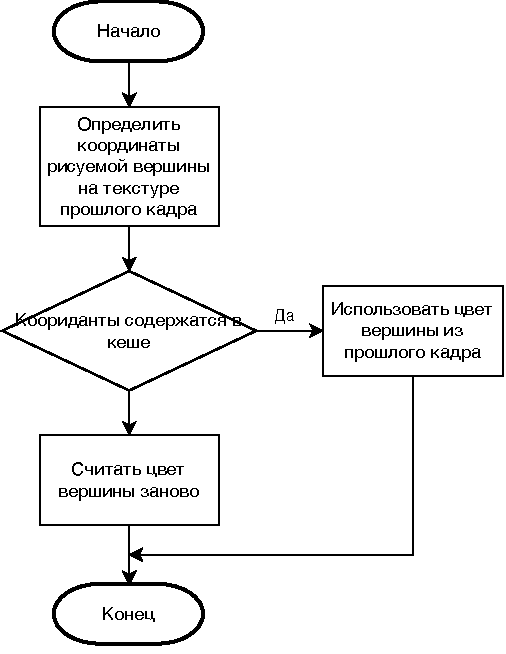
\includegraphics[width=90mm]{inc/pdf/rrc}
	\caption{Схема алгоритма кеширования обратной репроекции}
	\label{img:rrc}
\end{figure}

В листинге~\ref{lst:reproject} приведен псевдокод процерования точки в пространстве 
текущего кадра на пространство другого кадра.

\begin{lstlisting}[caption={Проецирование одного кадра на другой},label={lst:reproject},frame=single]
vec4 p = projection_matrix * inverse(previous_view_matrix) * vec4(position, 1.0);
p = p.xyz / p.w;
vec2 previous_uv = vec2((p.x / 2.0) + 0.5, (p.y / 2.0) + 0.5);
\end{lstlisting}

\section*{Вывод}

В данном разделе были описаны особенности алгоритмов для выполнения
на графических процессорах, алгоритмы и структуры данных, выбранные 
и разработанные для решения поставленной задачи. 
